\section{Functional Requirements}
\subsection{Introduction}

\subsubsection{Scope}
The \#YOCO utility should be implemented within the current AutoMart system and should not replace it. The subsystem needs to provide features that will help AutoMart reduce the number of poor and irrelevant advertisements on their website.

In this regard, the utility acts as a firewall that blocks bad quality images from entering the database while also validating that images that do pass as good quality, are well represented in the advertisement.

The system determines the image validity and quality by performing car detection, car coverage, blur and colour detection. Car detection is performed first as further tests and analysis require car location in the image in order to perform their own analysis. Car detection needs to check if the image contains a car. If the image contains a car, detection rating is set to one, and if no car is found detection rating is set to zero. Further tests are independent and can be conducted in any order. 

Car coverage calculates the area the car occupies in the image. Depending on the coverage percentage a value between zero and two is assigned to the coverage rating. Blur detection determines the image blurriness. Depending on the blurriness percentage a value between zero and two is assigned to the blur rating. Colour detection determines the colour of the car. AutoMart currently has sixteen colour buckets that are used to represent the colour of the car. The system calculate which colour bucket is the closest to the car's colour.

Finally the final image rating is calculated by adding detection rating, coverage rating and blur rating. The image rating and colour of the car are returned to the client side where further decisions can be performed based on clients preference. 

\pagebreak
\subsubsection{Limitations}
The system will not always be able to determine the correct colour of the car as aspects such as lighting, shadow and angle make it difficult to determine the colour correctly.

\subsubsection{Exclusions}
The system should only be implemented to work with cars and should not cater for the existence of any other vehicles such as motorcycles and trucks. The system is not able to determine the make and the model of the car. The recognition of different makes of the cars could be implemented in the future. However the recognition of models is not as no possible solution was found.

\subsection{Required Functionality}
\begin{figure}[h!]High Level Use Case Diagram.
  \centering
	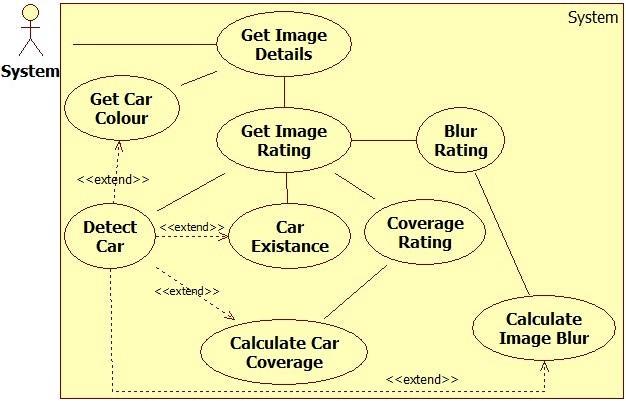
\includegraphics{HighLevelUseCase.jpg}
\end{figure}

\subsection{Use Cases}
\begin{tabular}{ | l | l |}
	\hline
  	\multicolumn{2}{| c |}{\textbf{Get Image Details}} \\
  	\hline
  	\multicolumn{2}{| c |}{Analyse the image and return its details.}\\
	\hline
	Priority & Critical \\	
  	\hline
  	Pre-Conditions & A valid image needs to be provided.\\
  	\hline
 	Post-Conditions & The image details acquired and returned.\\
  	\hline
\end{tabular}\\
\\
\\
\begin{tabular}{ | l | l | }
	\hline
  	\multicolumn{2}{| c |}{\textbf{Get Image Rating}} \\
  	\hline
  	\multicolumn{2}{| c |}{Calculates the image rating based on car existence, blur rating and coverage rating.}\\
	\hline
	Priority & Important \\	
  	\hline
  	Pre-Conditions & Blur rating, coverage rating and car existence need to be completed prior to execution.\\
  	\hline
 	Post-Conditions & Valid rating stored in the image details.\\
  	\hline
\end{tabular}\\
\\
\\
\begin{tabular}{ | l | l | }
	\hline
  	\multicolumn{2}{| c |}{\textbf{Car Existence}} \\
  	\hline
  	\multicolumn{2}{| c |}{Check if the car was found. Assign a rating of one for car detected and zero for no car detected.}\\
	\hline
	Priority & Important \\	
  	\hline
  	Pre-Conditions & Detect car needs to be completed prior to execution.\\
  	\hline
 	Post-Conditions & N/A\\
  	\hline
\end{tabular}\\
\\
\\
\begin{tabular}{ | l | l | }
	\hline
  	\multicolumn{2}{| c |}{\textbf{Coverage Rating}} \\
  	\hline
  	\multicolumn{2}{| c |}{Assigns a rating on scale zero to two based on the car coverage percentage.}\\
	\hline
	Priority & Important \\	
  	\hline
  	Pre-Conditions & The calculate car coverage has been executed.\\
  	\hline
 	Post-Conditions & N/A\\
  	\hline
\end{tabular}\\
\\
\\
\begin{tabular}{ | l | l | }
	\hline
  	\multicolumn{2}{| c |}{\textbf{Blur Rating}} \\
  	\hline
  	\multicolumn{2}{| c |}{Assigns rating on scale zero to two depending on the blur value and stores it in the image details .}\\
	\hline
	Priority & Important \\	
  	\hline
  	Pre-Conditions & The calculate blur has been executed.\\
  	\hline
 	Post-Conditions & N/A\\
  	\hline
\end{tabular}\\
\\
\\
\begin{tabular}{ | l | l | }
	\hline
  	\multicolumn{2}{| c |}{\textbf{Calculate Car Coverage}} \\
  	\hline
  	\multicolumn{2}{| c |}{Calculates the percentage the car occupies in the image.}\\
	\hline
	Priority & Important \\	
  	\hline
  	Pre-Conditions & Car must be detected in the image. Region of rectangle must be over image bounds.\\
  	\hline
 	Post-Conditions & Car coverage value successfully stored in the image details.\\
  	\hline
\end{tabular}\\
\\
\\
\begin{tabular}{ | l | l | }
	\hline
  	\multicolumn{2}{| c |}{\textbf{Calculate Blur}} \\
  	\hline
  	\multicolumn{2}{| c |}{Blur detection grey scales the image. loops through all the grey pixels, the difference between the pixel and all the adjacent pixels is calculated by taking the absolute value of the difference between any of the R,G or B channels. If the difference is over a certain threshold, a counter is incremented.  The count represents the blur value of the image and stores in the image details.}\\
	\hline
	Priority & Important \\	
  	\hline
  	Pre-Conditions & Image must exist.\\
  	\hline
 	Post-Conditions & Image blur value successfully stored in the image details.\\
  	\hline
\end{tabular}\\
\\
\\
\begin{tabular}{ | l | l | }
	\hline
  	\multicolumn{2}{| c |}{\textbf{Get Car Colour}} \\
  	\hline
  	\multicolumn{2}{| c |}{Calculates the colour of the car.}\\
	\hline
	Priority & Important \\	
  	\hline
  	Pre-Conditions & Car must be detected in the image.\\
  	\hline
 	Post-Conditions & Stores the colour of the car in the image details.\\
  	\hline
\end{tabular}\\
\\
\\
\begin{tabular}{ | l | l | }
	\hline
  	\multicolumn{2}{| c |}{\textbf{Detect Car}} \\
  	\hline
  	\multicolumn{2}{| c |}{Using Haar Cascades, an image is run through a car classifier that looks for features and well-known regions (such as a dark circle lower down in the image that may represent a wheel). All of these features are then combined into one larger rectangle that encapsulates the entire car.}\\
	\hline
	Priority & Critical \\	
  	\hline
  	Pre-Conditions & Image and classifiers are available.\\
  	\hline
 	Post-Conditions & Car existence status successfully stored in the image details.\\
  	\hline
\end{tabular}\\
\pagebreak
\subsection{Process Specifications}
\begin{figure}[h!]
  \caption{Activity diagram of FindBoundingBox}
  \centering
	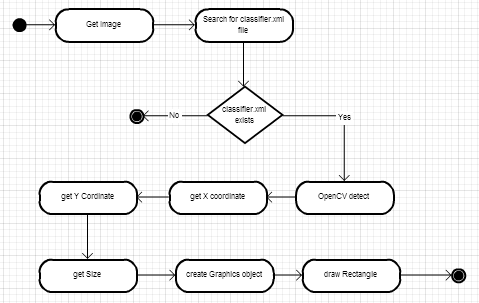
\includegraphics{activity.PNG}
\end{figure}
